\documentclass{article}
\usepackage[utf8]{inputenc}
\usepackage{geometry}
\geometry{
	a4paper,
	total={170mm,257mm},
	left=20mm,
	top=20mm,
}
\usepackage{graphicx}
\graphicspath{{images/}}
\usepackage{svg}
\usepackage{titling}
\usepackage[american,RPvoltages]{circuiTikz}
\usepackage{tikz, tikz-cd}
\usepackage{pgfplots}
\usepackage{siunitx}
\usepackage{float}
\usepackage{enumitem}
\usepackage{amsmath,amsfonts,stmaryrd,amssymb} % Math packages
\usepackage{tcolorbox}
\usepackage{pdfpages}
\title{Multiplicador de capacitancia}
\author{Rodrigo}
\date{Agosto 2024}


\usepackage{fancyhdr}
\fancypagestyle{plain}{%  the preset of fancyhdr 
	\fancyhf{} % clear all header and footer fields
	\fancyfoot[L]{\thedate}
	\fancyhead[L]{Multiplicador de capacitancia}
	\fancyhead[R]{\theauthor}
}
\makeatletter
\def\@maketitle{%
	\newpage
	\null
	\vskip 1em%
	\begin{center}%
		\let \footnote \thanks
		{\LARGE \@title \par}%
		\vskip 1em%
		%{\large \@date}%
	\end{center}%
	\par
	\vskip 1em}
\makeatother


%\usepackage[color=red!20]{draftwatermark}
%\SetWatermarkText{CONFIDENTIAL\\COPY}
%\SetWatermarkScale{3}

\usepackage{lipsum}  
%\usepackage{cmbright}
%\usepackage{mathpazo}
%\usepackage{ccfonts,eulervm}
 \usepackage[T1]{fontenc}
 \usepackage{ccfonts}
%\usepackage[math]{anttor}
%\usepackage{antpolt}
 %\usepackage{fouriernc}
%\usepackage[utopia]{mathdesign}
%---------------------------------------------------
\tikzset{flipflop myRS/.style={flipflop,
		 flipflop def={t1=R, t3=S, t6=Q, t4={\ctikztextnot{Q}}, tu={\ctikztextnot{RST}}, nu=1, n4=1 }}
	}
	
\tikzset{flipflop myFFRS/.style={flipflop,
		flipflop def={t1=R, t3=S, t6=Q, t4={\ctikztextnot{Q}}, n4=1 }}
}
%---------------------------------------------------
\setlength\parindent{0pt}


\begin{document}
	
\maketitle
	
\noindent\begin{tabular}{@{}ll}
Author & \theauthor\\
\end{tabular}
	
\section*{Introducción}
El circuito con amplificador operacional de la siguiente figura se conoce como \textit{multiplicador de capacitancia}. Tal circuito se usa en tecnología de circuitos integrados para producir un múltiplo de una reducida capacitancia física $C$ cuando se necesita una gran capacitancia. El circuito de la figura 1 puede servir para multiplicar valores de capacitancia por un factor de hasta 1000. Por ejemplo, un capacitor de $\qty{10}{\pico \farad}$ puede comportarse como uno de $\qty{100}{\nano \farad}$.

\begin{figure}[H]
	\centering	
	\begin{tikzpicture}[scale=0.8]
		\ctikzset{bipoles/thickness=4}
		\ctikzset{monopoles/vcc/arrow={Stealth[width=6pt,length=9pt]}}
		\ctikzset{monopoles/vee/arrow={Stealth[width=6pt,length=9pt]}}
		\draw (0,0) node[op amp, anchor=out](OA1){};
		\draw (OA1.-) to[short] ++(-1,0) to[short] ++(0,2) coordinate (p1);
		\draw (p1) to [short] (p1 -| OA1.out) coordinate (p2) node[above]{$V_i$} -- (OA1.out);
		\draw (p2) to[R, *-*, l=$R_1$] ++(4,0) coordinate (p4) node[above]{$2$} to[short] ++(0,-2) to[short] ++(1,0) coordinate (p3);
		\draw (p3) node[op amp, anchor=-](OA2){};
		\draw (p4) to[R, l=$R_2$] (p4 -| OA2.out) coordinate (p5) -- (OA2.out) node[right]{$V_o$};
		\draw (OA1.+) to[short] ++(-1,0) coordinate (p6);
		\draw (p6) node[above]{$1$} to[short] ++(0,-3) coordinate (p7) to[C, l=$C$, f= $I_c$] (p7 -| OA2.out) to[short, -*] (OA2.out);
		\draw (p6) to[short, *-o, f_<=$I_i$] ++(-2,0) coordinate (in);
		\draw (in) to[open, -o, v=$v_i$] ++(0,-3) node[ground]{};
		\draw (OA2.+) to[short] ++(-1,0) to[short] ++(0,-1) node[ground]{};
		\draw[<-] (-6.5, -2) -- (-7.5,-2) node[right=3mm, above]{$Z_i$};
	\end{tikzpicture}
	\caption{Circuito básico de un multiplicador de capacitancia.}	
	\label{fig:figura1}
\end{figure}

El rpimer amplificador operacional funciona como un seguidor de tensión, en tanto que el segundo es un amplificador inversor. El seguidor de tensión aísla la capacitancia formada por el circuito a partir de la carga impuesta por el amplificador inversor. Puesto que no entra corriente a las terminales de entrada del amplificador operacional, la corriente de entrada $I_i$ fluye a través del capacitor de retroalimentación.

\section*{Análisis}
Al aplicar la LCK en el nodo 1 obtenemos

\begin{align}
	I_i(s) = I_c(s)
\end{align}

O bien

\begin{align}
	I_i(s) = sC\left[ V_i(s) - V_o(s) \right]
\end{align}

La aplicación de la LCK en el nodo 2 da como resultado

\begin{align}
	I_{R_1}(s) = I_{R_2}(s)
\end{align}

O bien

\begin{align}
	\frac{V_i(s) - 0}{R_1} = \frac{0-V_o(s)}{R_2}
\end{align}

Por lo tanto

\begin{align}
	V_o(s) = -\frac{R_2}{R_1}V_1(s)
\end{align}

La sustitución de la ecuación (5) en la ecuación (2) produce

\begin{align}
	I_i(s) &= sC\left[ V_i(s) + \frac{R_2}{R_1}V_1(s) \right] \nonumber \\
	I_i(s) &= sCV_i(s)\left[ 1  +\frac{R_2}{R_1} \right]
\end{align}

La impedancia de entrada es

\begin{align}
	Z_i(s) = \frac{V_i(s)}{I_i(s)} = \frac{1}{sC_{eq}}
\end{align}

Donde
\begin{tcolorbox}[colback=red!5!white,colframe=red!75!black,arc=0mm,boxrule=0mm,width=(\linewidth+0.5cm)]
	\begin{equation}
		C_{eq} = C \left(1 + \frac{R_2}{R_1}\right)
	\end{equation}
\end{tcolorbox}

Si despejamos $R_2$ de la ecuación (8) obtenemos

\begin{align}
	\frac{R_2}{R_1} = \frac{C_{eq}}{C} -1 
\end{align} 

\begin{tcolorbox}[colback=red!5!white,colframe=red!75!black,arc=0mm,boxrule=0mm,width=(\linewidth+0.5cm)]
	\begin{equation}
		R_2 = \left( \frac{C_{eq}}{C} - 1 \right)R_1
	\end{equation}
\end{tcolorbox}


Así, mediante una adecuada selección de valores de $R_1$ y $R_2$, se puede lograr que el circuito con amplificador operacional de la figura 1 produzca una capacitancia efectiva entre la terminal de entrada y tierra, la cual es un múltiplo de la capacitancia física C. El tamaño de la capacitancia efectiva está limitado prácticamente por la limitación de la tensión de salida invertida. De este modo, a mayor multiplicación de la capacitancia menor tensión de entrada permisible, para evitar que los amplificadores operacionales lleguen a la saturación.

\section*{Ejemplo 1}
Sea el cicuito de la figura 2, donde $R_1 = \qty{1}{\kilo \ohm}$ y $C_1 = \qty{1}{\nano \farad}$. Y sea además una señal cuadrada con una amplitud de $\qty{1}{\volt}$ a una frecuencia de $\qty{100}{\hertz}$

\begin{figure}[H]
	\centering	
	\begin{tikzpicture}[scale=0.8]
		\ctikzset{bipoles/thickness=4}
		\ctikzset{monopoles/vcc/arrow={Stealth[width=6pt,length=9pt]}}
		\ctikzset{monopoles/vee/arrow={Stealth[width=6pt,length=9pt]}}
		\draw (0,0) to[V, l=$v_i(t)$] ++(0,4) 
		      to[R, l=$R_1$] ++(6,0)
		      to[C, l=$C_1$] ++(0,-4)
		      to[short] (0,0);
		      
		\pgfplotsset{width=9cm,height=5cm,compat=1.18}
		\begin{axis}[xshift=10cm,
			yshift=0cm,
			clip=false,
			axis y line=left,
			axis x line=middle,
			xlabel=$t$,
			ylabel=$v_i(t)$, 
			axis y line= center,
			xmin=0,xmax=5,
			ymin=0,ymax=1.5,
			xtick={0,2,4},
			ytick={1},
			xticklabels={$0$,$T/2$,$T=\qty{10}{\milli \second}$},
			yticklabels={$1$},
			]
			\addplot+[line width=1pt,mark=none,const plot]
			coordinates {(0,1) (2,1) (2,0) (4,0)};
			%\addplot[color = black, dashed, thick] coordinates {(0.5,0) (0.5,-1)}; %vertical1
			%\addplot[color = black, dashed, thick] coordinates {(2,0) (2,-1)}; %vertical2
			%\draw[Stealth-] (0.5,-0.5) node[right=8.5mm]{$T$}-- (1,-0.5);
			%\draw[-Stealth] (1.5,-0.5) -- (2,-0.5);
		\end{axis}
	\end{tikzpicture}
	\caption{Circuito básico de un multiplicador de capacitancia.}	
	\label{fig:figura2}
\end{figure}

El voltaje en el capacitor está dado por

\begin{align}
	v_c(t) = v(\infty) + \left[ v(0) - v(\infty) \right]e^{-\frac{t}{\tau}}
\end{align}

Donde

\begin{subequations}
	\begin{align}
		v(0) &= 0 \label{second:a} \\
		v(\infty) &= 1 \label{second:b}
	\end{align}
\end{subequations}

Sustituyendo los valores de la ecuación (12) en (11) obtenemos

\begin{align}
	v_c(t) = 1 - e^{-\frac{t}{\tau}}
\end{align}

Donde

\begin{align}
	\tau = R_1C_1 = (1 \times 10^6)(1 \times 10^{-9}) = \qty{1}{\milli \second}
\end{align}

De esta manera, el voltaje en el capacitor es

\begin{align}
	v_c(t) = 1 - e^{-1000t}
\end{align}

El capacitor se carga al 99\% de su valor en aproximadamente 6 constantes de tiempo $(6\tau)$, a continuación, se muestra la gráfica de carga del capacitor.
	
\begin{figure}[H]
\centering	
\begin{tikzpicture}[scale=0.8]	
	\pgfplotsset{width=9cm,compat=1.18}
	\begin{axis}[xshift=9cm,
		yshift=-0.5,
		clip=false,
		axis y line=left,
		axis x line=middle, 
		xmin=0,xmax=0.006,
		ymin=0,ymax=1.2,
		xlabel=$\omega t$,
		%xtick={3.14,6.28},
		%xticklabels={$\pi\,$, $\,\,\,2\pi$},
		ytick={0.2,0.6,1},
		%yticklabels={$\sqrt{2}V$},
		]
		\addplot[smooth, magenta, mark=none, domain=0:0.006, samples=200] {1-exp(-1000*x)};
		\addplot[color = black, dashed, thick] coordinates {(0,1) (0.006,1)}; %vertical1
	\end{axis}
	
	\draw (9.4,6) node[above right, xshift=-20pt]{$v_c(t)$};
\end{tikzpicture}
\caption{Voltaje del capacitor para el circuito de la figura 2.}	
\label{fig:figura3}
\end{figure}

Suponga que se desea diseñar un circuito multiplicador de ganancia por 10. Es decir, si tenemos un capacitor $C = \qty{1}{\nano \farad}$, se deberán escoger los valores de $R_1$ y $R_2$ de manera que $C_{eq} = \qty{10}{\nano \farad}$.

Utilizamos la ecuación (9) para obtener la razón o cociente entre las resistencias

\begin{align}
	\frac{R_2}{R_1} &= \frac{C_{eq}}{C} - 1 \nonumber \\
	\frac{R_2}{R_1} &= 9 \nonumber
\end{align}

Si seleccionamos $R_1 = \qty{10}{\kilo \ohm}$, entonces $R_2 = \qty{90}{\kilo \ohm}$. El circuito se muestra en la figura 4.

\begin{figure}[H]
	\centering
	% trim=left botm right top
	
\includegraphics[clip, trim=0cm 10cm 0cm 10cm, width=\textwidth]{figure1}
	\caption{Circuito esquemático de un multiplicador de capacitancia}	
	\label{fig:figura4}
\end{figure}

De la ecuación (5) tenemos que el voltaje de salida es

\begin{align}
	V_o(s) = -\frac{R_2}{R_1}V_i(s) = -\frac{\qty{90}{\kilo \ohm}}{\qty{10}{\kilo \ohm}}(\qty{1}{\volt}) = -\qty{9}{\volt}
\end{align}

Con esto nos aseguramos que el amplificador operacional no alcanza a saturarse. La constante de tiempo será ahora de 

\begin{align}
	\tau = RC_{eq} = (1 \times 10^{3})(10 \times 10^{-9}) = \qty{10}{\milli \second}
\end{align}

Así, la nueva ecuación para el voltaje en el capacitor es:

\begin{align}
	v_c(t) = 1 - e^{-100t}
\end{align}


Por lo que ahora al capacitor le tomará cargarge aproximadamente $6\tau = \qty{60}{\milli \second}$, como se muestra en la figura 5.

\begin{figure}[H]
	\centering	
	\begin{tikzpicture}[scale=0.8]	
		\pgfplotsset{width=9cm,compat=1.18}
		\begin{axis}[xshift=9cm,
			yshift=-0.5,
			clip=false,
			axis y line=left,
			axis x line=middle, 
			xmin=0,xmax=0.06,
			ymin=0,ymax=1.2,
			xlabel=$\omega t$,
			%xtick={3.14,6.28},
			%xticklabels={$\pi\,$, $\,\,\,2\pi$},
			ytick={0.2,0.6,1},
			%yticklabels={$\sqrt{2}V$},
			]
			\addplot[smooth, magenta, mark=none, domain=0:0.06, samples=200] {1-exp(-100*x)};
			\addplot[color = black, dashed, thick] coordinates {(0,1) (0.06,1)}; %vertical1
		\end{axis}
		
		\draw (9.4,6) node[above right, xshift=-20pt]{$v_c(t)$};
	\end{tikzpicture}
	\caption{Voltaje del capacitor para $v_c(t) = 1 - e^{-100t}$}	
	\label{fig:figura5}
\end{figure}

En la siguiente figura se muestra una comparación de los dos tiempos de carga para el capacitor

\begin{figure}[H]
	\centering	
	\begin{tikzpicture}[scale=0.8]	
		\pgfplotsset{width=9cm,compat=1.18}
		\begin{axis}[xshift=9cm,
			yshift=-0.5,
			clip=false,
			axis y line=left,
			axis x line=middle, 
			xmin=0,xmax=0.06,
			ymin=0,ymax=1.2,
			xlabel=$\omega t$,
			%xtick={3.14,6.28},
			%xticklabels={$\pi\,$, $\,\,\,2\pi$},
			ytick={0.2,0.6,1},
			%yticklabels={$\sqrt{2}V$},
			]
			\addplot[smooth, blue, mark=none, domain=0:0.06, samples=200] {1-exp(-1000*x)};
			\addplot[smooth, magenta, mark=none, domain=0:0.06, samples=200] {1-exp(-100*x)};
			\addplot[color = black, dashed, thick] coordinates {(0,1) (0.06,1)}; %vertical1
		\end{axis}
		
		\draw (9.4,6) node[above right, xshift=-20pt]{$v_c(t)$};
	\end{tikzpicture}
	\caption{Comparación entre los diferentes tiempos de carga del capacitor}	
	\label{fig:figura6}
\end{figure}

\begin{figure}[H]
	\centering
	% trim=left botm right top
	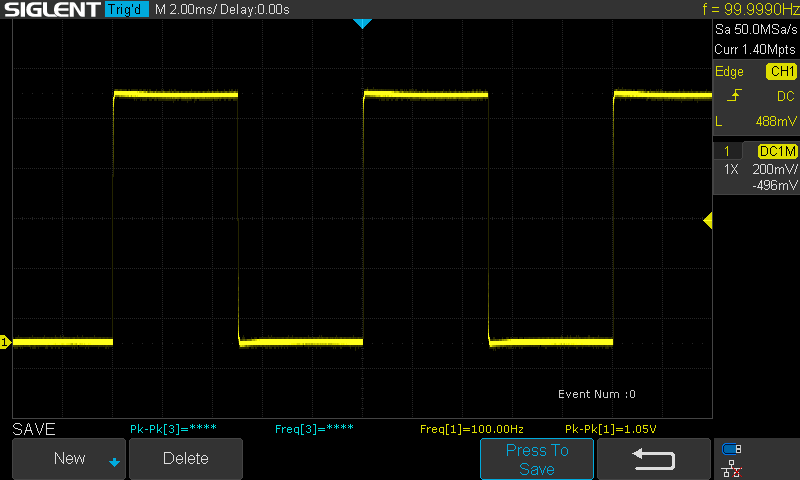
\includegraphics[scale=0.6]{SDS00008}
	\caption{Señal de entrada del circuito}	
	\label{fig:figura7}
\end{figure}

\begin{figure}[H]
	\centering
	% trim=left botm right top
	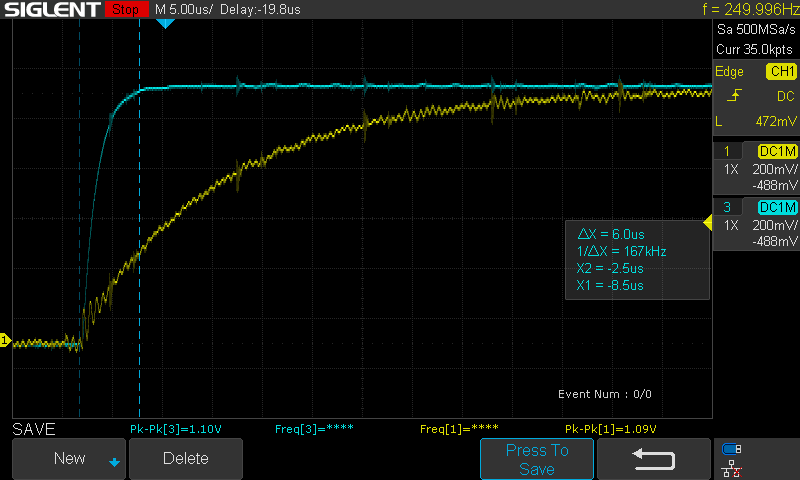
\includegraphics[scale=0.6]{SDS00010}
	\caption{Comparación de las señales de salida. Azul circuito simple, Amarillo circuito multiplicador de capacitancia.}	
	\label{fig:figura8}
\end{figure}

\begin{figure}[H]
	\centering
	% trim=left botm right top
	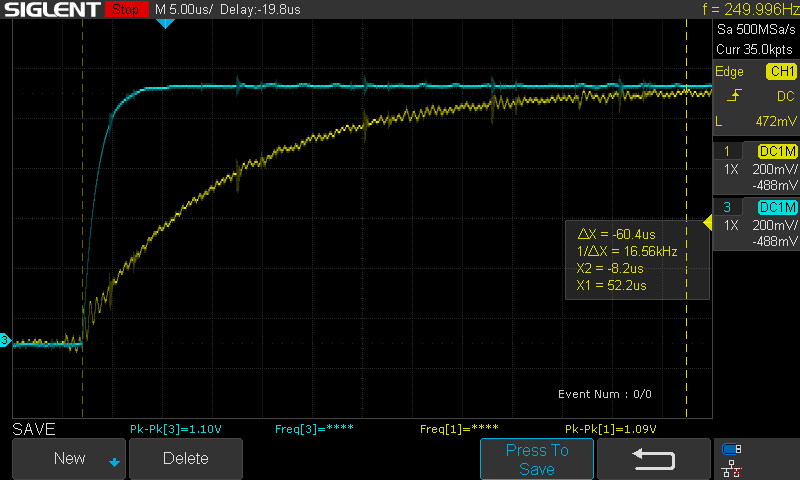
\includegraphics[scale=0.6]{SDS00009}
	\caption{Comparación de las señales de salida. Azul circuito simple, Amarillo circuito multiplicador de capacitancia.}	
	\label{fig:figura9}
\end{figure}

\end{document}